To obtain reliable models, one must both choose or create a training set
carefully and study the impact of various algorithm parameters on the error.
Although the title of this section suggests final steps of confirming a model's
usefulness for predictions, what follows is more of a diagnostic exercise. 
In practice, these analyses can be used for both purposes.

\gls{ML} algorithms are heavily dependent on the training inputs and algorithm
parameters given to them, such as training set sizes, regularization, number of
features in the training set, optimization parameters, etc.  From the results
shown in Section \ref{sec:statmodel}, it is clear there is room for
improvement.  To evaluate these input and parameter variations, diagnostic
plots show the errors between the predicted burnup values and the actual burnup
values with respect to some variable on the \textit{x}-axis.  As previously
introduced in Section \ref{sec:optvalid}, the prediction errors are compared to
the training error to understand the generalization strength. These two errors
are plotted with respect to training set size (learning curves) and the
algorithm parameters governing model complexity (validation curves) to provide
insight into the model fitness. 

In addition to \gls{ML} best practices, another layer of comparison is
added here.  Because it is difficult to ensure consistently representative
testing data, the accuracy of a learned model should not depend on only one
testing set.  The learned model's accuracy is better estimated by using a
validation set. Here, this is implemented as \textit{k}-fold cross-validation,
introduced in Section \ref{sec:selectass}. This work includes both the testing
error (using the testing set described in Section \ref{sec:training}) and
5-fold cross-validation error. The predetermined testing set will allow for
comparison against the previous work it was obtained from
\cite{dayman_feasibility_2013}, but it is assumed that cross-validation will
provide a better indication of model performance because the entirety of the
training set has also been tested. 

\begin{figure}[!htb]
    \centering
    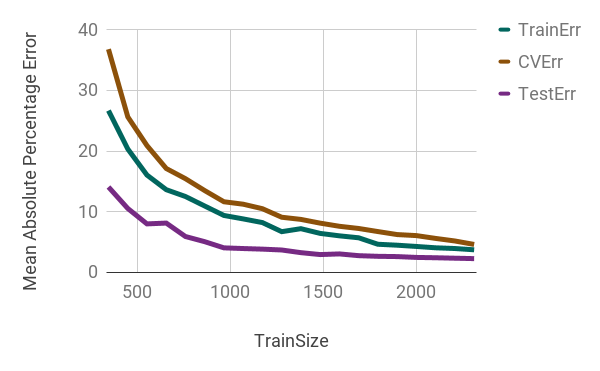
\includegraphics[width=\linewidth]{./chapters/demo_method/lc1.png}
    \caption{\acrshort{SVR} Learning Curve for Burnup Prediction, $TrainSet\ Size = 2313$}
    \label{fig:lc1}
\end{figure}

The learning curves are obtained as follows, shown in Figure \ref{fig:lc1}.
For a given (randomly chosen) training set size between 15 and 100\% of the
total data set, training and prediction rounds were performed for each. The
testing error scenario performs this $n=10$ times and averages those results.
The \textit{k} in \textit{k}-fold for cross-validation was chosen to be $5$.
\todo{dicuss over/under training}

\begin{figure}[!htb]
    \centering
    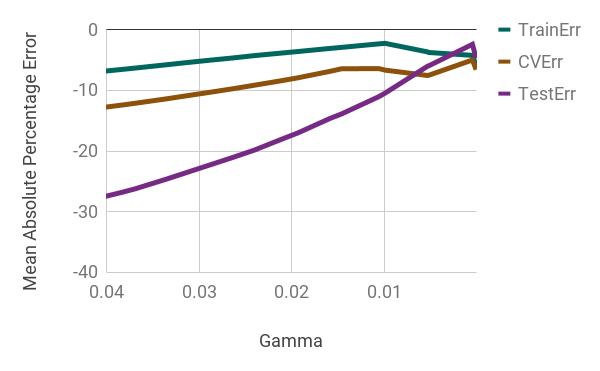
\includegraphics[width=\linewidth]{./chapters/demo_method/vc1.png}
    \caption{\acrshort{SVR} Validation Curve for Burnup Prediction, $\gamma = 0.001$}
    \label{fig:vc1}
\end{figure}

The validation curves are obtained as follows, shown in Figure \ref{fig:vc1}.
The $\gamma$ parameter in \gls{SVR} was varied from $10^{-4} -- 10^{-2}$.
Training and prediction rounds were carried out for each value of $\gamma$ with
the number of folds set to $5$ and the number of trials performed set to $10$.
This was also done for the $C$ parameter, varied from $10^{-2} -- 10^{5}$.
%Note that in Figure \ref{fig:vc1} the domain has been decreased to show the
%features close to the \textit{y}-axis.
Training and prediction rounds were performed for different $\gamma$ values in
this range.  Again, the testing and cross-validation errors are both used as
described above. As with Figure \ref{fig:lc1}, determining the robustness to
over- or undertraining is difficult here although there is possibly a minimum
at $\gamma=0.001$.  
\todo{Check NN, RR, and SVR-C LCs and VCs}

Although there is no example behavior of Figure \ref{fig:lc1}'s peculiar
learning curve in Figure \ref{fig:learning}, the curves mimic the squared bias
curve from Figure \ref{fig:bvtradeoff}. This suggests that the bias in the
model is much higher than the variance.  Next, the testing error is lower than
the training error; this should never be the case, and indicates an issue with
the systematically chosen testing set.  While the cross-validation error is
correctly higher than the training error, it follows along in parallel,
producing no information on model fitness other than confirming a very high
bias.  It is presumed this is not the fault of the algorithms, but the training
set itself.  It is likely covering too small of a range of the simulation
space.

Additionally, Figure \ref{fig:vc1}'s validation curve shows the testing error
dropping below the training error for extremely small $\gamma$, around where a
minimum might be.  Since the model suffers from high bias, no amount of model
complexity can be optimized. The resolution to the underfitting is discussed in
Section \ref{sec:prep}.


